\section{Strings}\label{sec:strings}
Heutzutage ist es schon fast undenkbar und unmöglich ein Programm ohne \emph{Strings} zu
schreiben. Sie sind ein fester Bestandteil, bei so gut wie jeder höheren Programmiersprache,
geworden. Viele Programmierer sehen diese deswegen als etwas sehr leichtgewichtiges. Dies kommt
daher, dass Strings genauso behandelt werden wie primitive Datentypen, wie zum Beispiel \emph{int}
oder \emph{char}. Jedoch wäre es Fatal anzunehmen, dass Operationen mit \emph{Strings} genauso
effizient
geschehen, wie bei den primitiven Datentypen. Dies zeigt auch das folgende Zitat:

\begin{zitat}
    Strings are convenient because they automatically grow as needed to hold their contents. By
    contrast, C library functions (strcat(), strcpy(), etc.) act on fixed-size character arrays.
    To implement this flexibility, strings are allocated dynamically. Dynamic allocation is
    expensive compared to most other C++ features, so no matter what, strings are going to show
    up as optimization hot spots \cite{OptimizedC++}
\end{zitat}

\subsection{Probleme mit Strings}\label{subsec:stringprobleme}
\emph{Strings} ziehen viele Probleme mit sich, jedoch sind die zwei Größten Probleme die
\emph{Strings} mit sich ziehen sind folgende:

\begin{itemize}
    \item \emph{Strings} werden auf dem \emph{Heap} gespeichert, was, wie im Kapitel
    \emph{\nameref{sec:speicherman}} gezeigt ein sehr Teurer Prozess ist.
    \item Dadurch dass \emph{Strings} wie primitive Datentypen behandelt werden, verursachen
    \emph{Strings} viele Kopiervorgänge, was, wie im Kapitel \emph{\nameref{sec:kopieren}} sehr
    suboptimal ist.
\end{itemize}

Um zu Demonstrieren, wie Problematisch diese zwei Punkte tatsächlich sind, soll die \emph{String}
klasse, die im laufe dieses Papers vorgestellt wurde um die \emph{+} und \emph{=} Operatoren
erweitert werden, wie im folgenden gezeigt:
\newpage
\begin{lstlisting}[
    caption={String-Operatoren},
    label=lst:StringOperatoren,
    language=C++,frame=tlrb]
	String& operator=(const String& other) noexcept {
		printf("Copied via =\n");
		if (this == &other)
			return *this;

		delete[] m_Data;
		m_Size = other.m_Size;
		m_Data = new char[m_Size + 1];
		memcpy(m_Data, other.m_Data, m_Size + 1);
		return *this;
	}

	String& operator+(const String& other) noexcept {
		this->operator+(other.m_Data);
	}

	String& operator+(const char* other) noexcept {
		printf("Copied via +\n");
		String temp = *this;

		delete[] m_Data;
		int other_Size = strlen(other);
		m_Size = temp.m_Size + other_Size;
		m_Data = new char[m_Size + 1];

		int i = 0;
		for (int j = 0; j < temp.m_Size; ++j, ++i)
			m_Data[i] = temp.m_Data[j];
		for (int j = 0; j < other_Size; ++j, ++i)
			m_Data[i] = other[j];

		m_Data[m_Size] = 0;
		return *this;
	}
\end{lstlisting}

Damit die beiden Operatoren so funktionieren, wie sie sollen, muss der Speicher für \emph{m\_Data}
mittels \emph{new} vergrößert werden. Darauf hin müssen die Daten, entweder mit Standard Funktionen
wie \emph{memcpy} oder mit simplen \emph{for-schleifen}, kopiert werden.
\newline
\newline
Da nun die beiden Operatoren zur Verfügung stehen, kann nun mit der folgenden Sequenz, die
Problematik zur Schau gestellt werden. Hierfür wird außerdem noch der \emph{new} Operator
überschrieben um später zu überprüfen, wie oft die Funktion aufgerufen wurde.

\begin{lstlisting}[
    caption={String-Operationen},
    label=lst:StringOperationen,
    language=C++,frame=tlrb]
static uint64_t Allocations = 0;

void* operator new(size_t size) {
	++Allocations;
	return malloc(size);
}

int main(int argc, char** argv)
{
	String demo = String("Hello") + " World" + "!";
	std::cout << "New called " << Allocations << " times" << std::endl;
	std::cin.get();
}
\end{lstlisting}
Wird die Sequenz betrachte, dann ist dies nichts Weltbewegendes, jedoch resultiert diese Sequenz
schließlich in diesen Output:

\begin{lstlisting}[
    caption={Ausgabe des String-Programms},
    label=lst:StringProgramm,
    language=C++]
Created
Copied via +
Copied
Copied via +
Copied
Copied
New called 6 times
\end{lstlisting}

Tatsächlich wurde für dieses doch sehr simple Programm Sechs mal der \emph{new} Operator
aufgerufen. Eine Optimierungsansatz für dieses Problem, sind \emph{\nameref{sec:move}}, die im
späteren Verlauf dieses Papers noch besprochen werden, jedoch ist dieses Verhalten aus Sicht der
Performance inakzeptabel und der Einsatz von \emph{Strings} sollte auf ein nötigstes beschränkt
werden.

\subsection{String Optimierungen}
Wie im Unterkapitel \emph{\nameref{subsec:stringprobleme}} zu sehen war, bringen \emph{Strings}
einige Probleme hinsichtlich der Performance mit sich. Jedoch ist die Tatsache, dass
\emph{Strings} Performance Probleme mit sich ziehen kein geheimnis und weit bekannt. Deswegen
wird städig versucht \emph{Strings} performanter zu machen. Im folgenden werden aufgrund dessen
einige \emph{String} Optimierungen betrachtet, die im laufe der Jahre in den C++ standart
hinzugefügt wurden.
\newline
\subsubsection{Small String Optimization}
Natürlich ist die \emph{std::string} klasse aus dem C++ standart wesentlich Komplexer als die
eigen Implementierte \emph{String} klasse aus diesem Paper und bietet auch mehr Features. So auch
wie das Feature names \emph{Small String Optimization}, welche mit \emph{C++11} in den C++
standart kam. Wie in diesem Kapitel zu sehen war, müssen \emph{Strings} dynamisch auf dem
\emph{Heap} gespeichert werden. Durch \emph{Small String Optimization} werden \emph{Strings}, die
eine bestimmte Anzahl an Charakter nicht überschreiten, um genau zu sein, nicht größer als \emph{15}
Charakter, nicht auf dem \emph{Heap} sondern auf dem \emph{Stack} gespeichert. Dies ist durch die
folgende Demonstration zu erkennen:

\begin{lstlisting}[
	caption={Small String Optimization},
	label=lst:SmallString,
	language=C++,frame=tlrb]
int main(int argc, char** argv)
{
	std::string string1 = "Hallo";
	std::cout << string1 << ": New called " << Allocations << " times" << std::endl;

	Allocations = 0;

	std::string string2 = "Hallo das ist eine Demo";
	std::cout << string2 << ": New called " << Allocations << " times" << std::endl;

	//Output
	//Hallo: New called 0 times
	//Hallo das ist eine Demo: New called 1 times
}
\end{lstlisting}
\newline
\subsubsection{std::string\_view}
Mit \emph{C++17} wurde \emph{std::string\_view} in den C++ standart hinzugefügt und ermöglicht es
Programmierern, eine \emph{view} in einem \emph{String} zu bekommen. Eine \emph{view} sorgt
dafür, dass in einem schon vorhandenen string reingeschaut werden kann. Wird nun das Beispiel
betrachte, das ein \emph{Substring} von einem \emph{String} benötigt wird, dann muss für diesen
\emph{Substring} ein eigener \emph{Buffer} auf dem \emph{Heap} erzeugt werden, um dann den Teil
zu kopieren. Mit hilfe von \emph{std::string\_view} ist es nicht nötig, einen seperaten
\emph{Buffer} zu erzeugen, sondern es wird lediglich auf die Adresse des \emph{Strings} gezeigt
und eine Anzahl an \emph{Bytes} übergeben, um den Teil des \emph{Substrings} zu definieren.
\newline
\subsubsection{Reserve}
Die \emph{Reserve} funktion ist keine eigenheit von \emph{std::string}, jedoch kann diese
Funktion genau so gut auch für \emph{Strings} benutzt werden. Mit \emph{Reserve} kann Speicher
auf dem \emph{Heap} reserviert werden, das bedeutet, dass wenn die Anzahl der Bytes bekannt ist,
ist es nicht von nöten jedesmal nach einer Operation, mehr speicher anzufordern, sondern einmal
diese \emph{Bytes} zu reservieren und die Daten dann einfach reinzuschreiben. Angenommen, es
seien in einer \emph{Liste} beliebig viele \emph{Strings} vorhanden, und diese \emph{Strings}
sollen in  einem \emph{String} zusammen gefügt werden. Dann ist es tatsächlich Performanter,
zuerst die gesamten \emph{Bytes} zu ermitteln, die Anzahl an \emph{Bytes} für den \emph{String} zu
reservieren und am ende erst die einzelnen \emph{Strings} zu vereinen. Im folgenden wird ein
Diagramm gezeigt, welches den Unterschied mit und ohne \emph{Reserve} zeigt:
\begin{figure}[h]
	\centering
	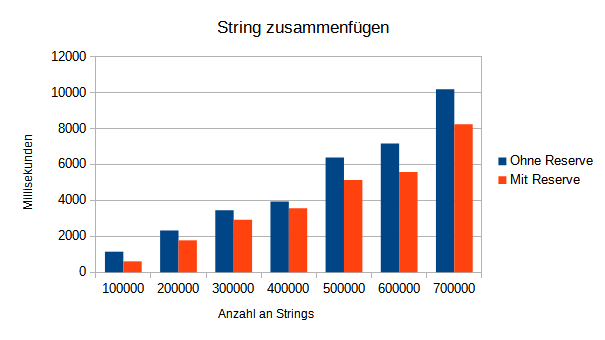
\includegraphics[width=0.5\textwidth]{bilder/StringReserve}
	\caption[StringsZusammenfügen]{Strings zusammenfügen}
	\label{img:StringsZusammenfügen}
\end{figure}